\documentclass[final,hyperref={pdfpagelabels=false}]{beamer}
\mode<presentation>{\usetheme{Wernecke_bright}}
\usepackage[orientation=portrait,size=a0,scale=1.4,debug]{beamerposter}
\usepackage[english]{babel}
\usepackage[utf8]{inputenc}
\graphicspath{{./images/}}
\usepackage{wrapfig}

\setbeamertemplate{caption}[numbered]
% packages and settings %%%%%%%%%%%%%%%%%%%%%%%%%%%%%%%%%%%%%%%%%%%%%%%%%%%%%%%%%%%%%%
% \usepackage{grffile}
\boldmath	

% PDF and title settings %%%%%%%%%%%%%%%%%%%%%%%%%%%%%%%%%%%%%%%%%%%%%%%%%%%%%%%%%%%%%
\title{Clique encoding in recurrent neural networks} %\\[0.2\baselineskip]with a second line
\author[varriale@itp.uni-frankfurt.de]{Emanuele Varriale, Claudius Gros}
\institute{Institute for Theoretical Physics, Goethe University, Frankfurt am Main, Germany}
\date{\today}
 
%%%%%%%%%%%%%%%%%%%%%%%%%%%%%%%%%%%%%%%%%%%%%%%%%%%%%%%%%%%%%%%%%%%%%%%%%%%%%%%%%%%%%%

\begin{document}

\begin{frame}

\begin{columns}
	
	% ---------------------------------------------------------%
	% Set up a column 1
	\hfill
	\begin{column}{.30\textwidth}
		%\begin{beamercolorbox}[center,wd=\textwidth]{postercolumn}
		\begin{minipage}[T]{.95\textwidth}	% tweaks the width, makes a new \textwidth
		\parbox[t][\columnheight]{\textwidth}{

			%%% CONTENT of column 1 %%%
			%\vfill
			\begin{block}{Introduction}
			Internal brain activity is only modulated, not driven, by sensory input \cite{fiser2004modulation}. 
				
			Therefore the semantic learning that takes place in the brain is a result of the interaction of external sensory stimuli with an autonomously active network.
				
			Clique encoding is a form of sparse coding, that is backed up by experimental findings about real-time memory representation in the hippocampus \cite{lin2006clique}.
				
			For this reason we work with a network with competing cliques, where the activity ``flows'' from one clique to another, with a transient state dynamics.
				
			We propose a learning rule that correlates such transient states with sensory inputs from the bars and stripes problem, prompted by \cite{gros2010semantic}.
			\end{block}
			
			\vfill
			\begin{block}{Network architecture}
			The term clique comes from graph theory and it refers to maximal fully connected sub-graphs. 
			
			In a network formed by cliques with excitatory synapses within and inhibitory ones across, the dynamics is characterized by competing cliques. 
			
			An active clique inhibits every other, so that this is a stable state.
			
			We use networks as the one shown in Fig. \ref{fig:network}, in which activity can spread from one clique to any other.
						
			
			\begin{figure}
				\centering
				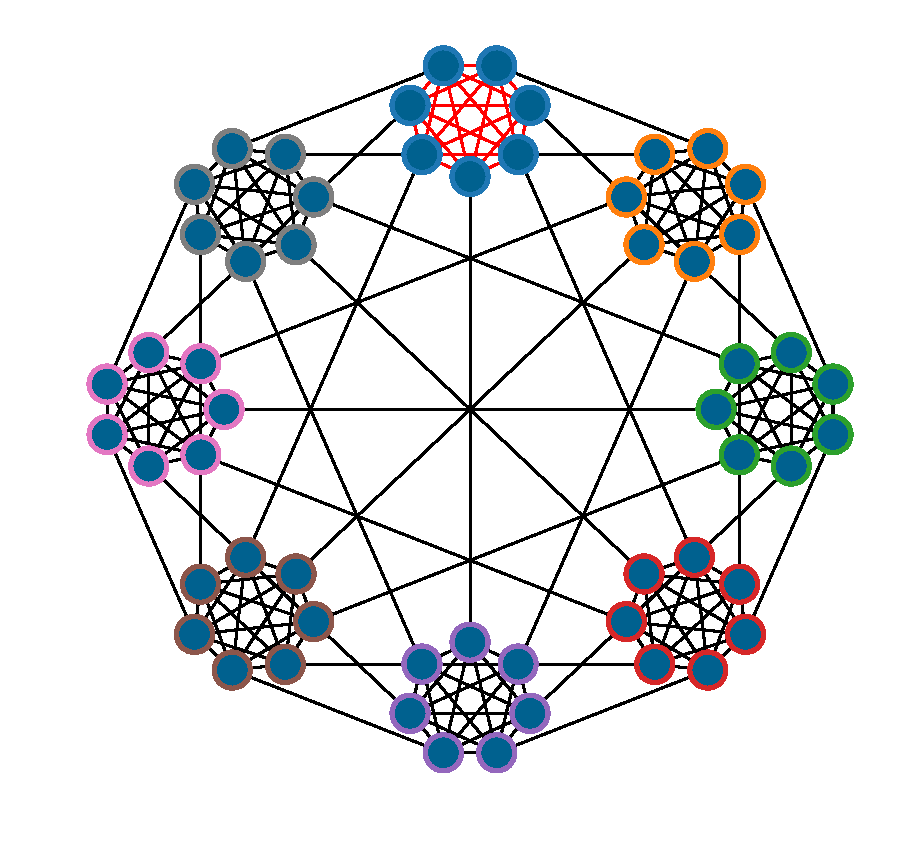
\includegraphics[width=.7\linewidth]{network2.pdf}
				\caption{An eight clique network, each with seven nodes. Only excitatory links are shown. Each node within a clique excite a neuron in a different clique. The network is completed with an inhibitory background of connections.}
				\label{fig:network}
			\end{figure}
			\end{block}		
							
			\vfill
			\begin{block}{Neuronal dynamics}
	 		The $j$-th neuron has membrane potential $x_j$, activity $y_j$ and receives excitatory and inhibitory input, respectively $E_j$ and $I_j$. The rate-encoding model is governed by the following equations:
			\begin{gather*}
				\tau_x \dot{x}_j = -x_j + E_j + I_j\\
				y_j = \sigma \left(x_k\right) = \frac{1}{1+\exp \left(-a x_k \right) } \\
				E_j = \sum_{k} w_{jk} y_k \\
				I_j = \sum_k z_{jk} y_k.
				\label{eq:neuron}
			\end{gather*}
			These equations lead to an attractor network, and the system rapidly relaxes to a stable state.
			
			Inserting a presynaptic reservoir variable the effective output changes, i.e.\ $y_k \rightarrow \tilde{y}_k$, and a transient state dynamics is obtained, as in Fig. \ref{fig:activity}.
			\begin{figure}
				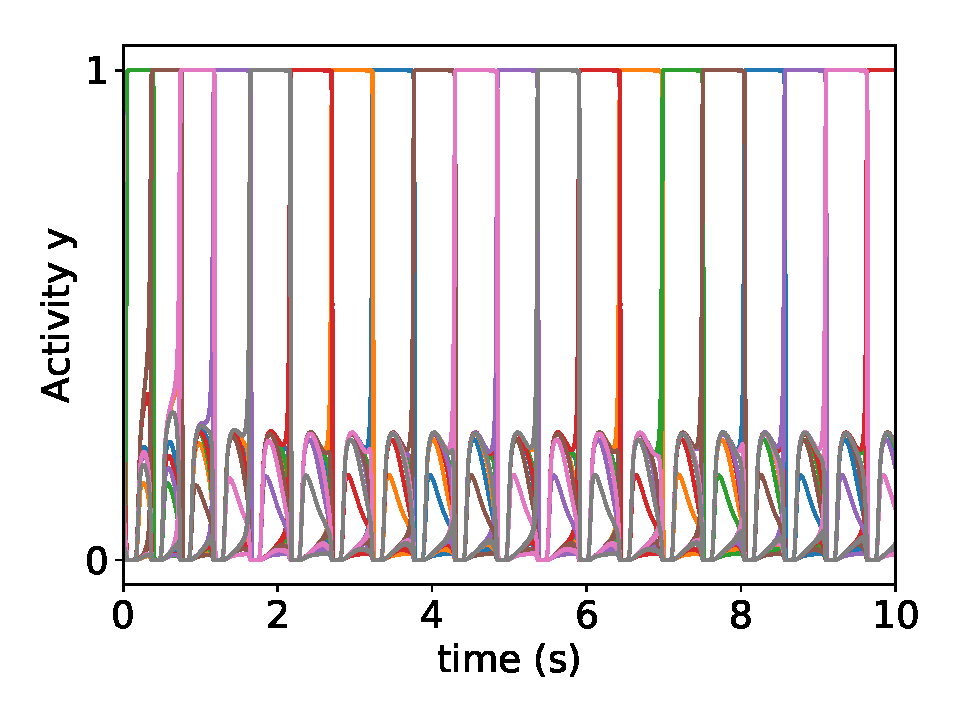
\includegraphics[width=.7\linewidth]{double_activity}
				\caption{Internal activity in the network shown above. The same colour is used for neurons belonging to the same clique, as shown in Fig. \ref{fig:network}.}
				\label{fig:activity}
			\end{figure}
			
			\end{block}
			
			
			
			%\vfill
			%\begin{emphblock}{Conclusions}
			%	\singleitem{That is really important to keep in mind.}
			%	\singleitem{Furthermore ...}
			%\end{emphblock}
			\vfill
			%%% END CONTENT of column 1 %%%

	 	} % end of parbox
		\end{minipage}
		%\end{beamercolorbox}
	\end{column}
	% ---------------------------------------------------------%
	% end of column 1
	%\hfil
	% ---------------------------------------------------------%
	% Set up a column 2
	\begin{column}{.64\textwidth}
		%\begin{beamercolorbox}[center,wd=\textwidth]{postercolumn}
		\begin{minipage}[T]{.95\textwidth}
		\parbox[t][\columnheight]{\textwidth}{

		%%% CONTENT of column 2 %%%
		%\vfill
		\begin{block}{Full depletion model}
			\begin{columns}
				\begin{column}[T]{.5\textwidth}
				\begin{figure}
					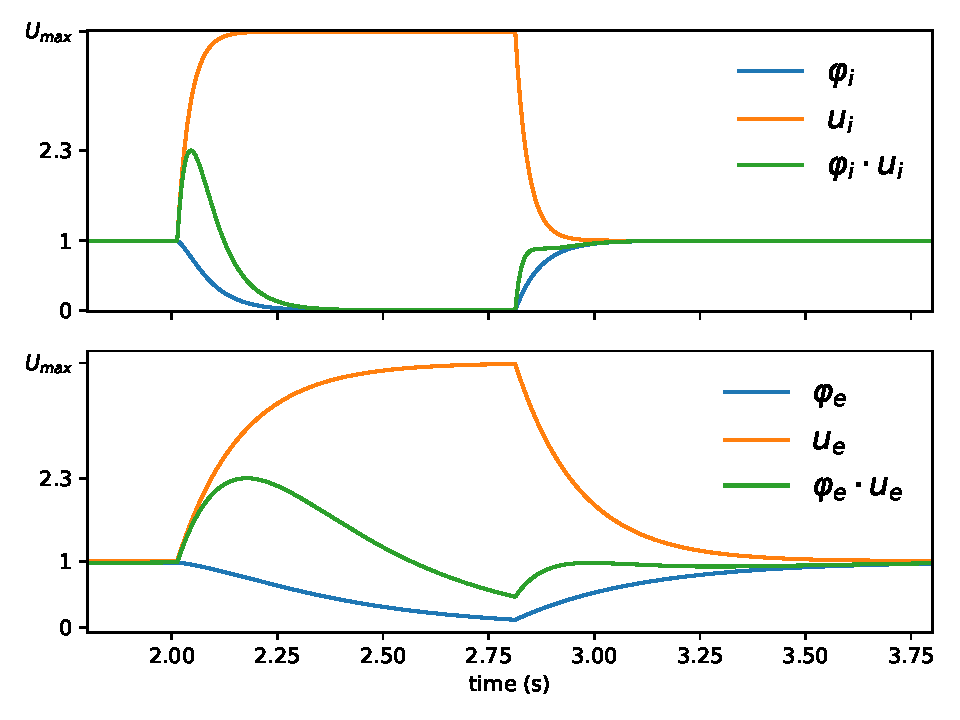
\includegraphics[width=1\linewidth]{double_depletion.pdf}
					\caption{Dynamics of the full depletion model, with high presynaptic activity.  Inhibitory short-term plasticity is faster than excitatory.}
					\label{fig:full_depletion}
				\end{figure}	
				\end{column}							
				
				\begin{column}[T]{.5\textwidth}
					Transient state dynamics requires winning clique states not to be stable. 
					
					This is achieved through the Full depletion model for short term plasticity, similar to the Tsodyks-Markram model \cite{tsodyks2008model}.
					
					Each neuron has a presynaptic reservoir variable that is completely depleted after sustained firing, more specifically presynaptic activity is modulated by two terms:
					\begin{itemize}
						\item $u_j$ represents the likelihood of neurotransmitter release, which increases with Ca$^{2+}$ traces,
						
						\item $\varphi_j$ represents the concentration of available vesicles, that depletes while firing.
					\end{itemize}
					The Full depletion model is given by:			
					\begin{gather*}
						\tilde{y}_j = y_j u_j \varphi_j \\
						\dot{u}_j = \frac{U_y -u}{T_u}, \quad U_y = 1 + \left( U_\text{max} -1 \right) y_j\\ 
						\dot{\varphi}_j = \frac{\varPhi_u - \varphi}{T_\varphi}, \quad \varPhi_u = 1- \frac{u y_j}{U_\text{max}} \\
						T^{\text{exc}} = 5 \cdot T^{\text{inh}}.
					\end{gather*}

				\end{column}
			\end{columns}
		\end{block}
		
		\begin{block}{Sensory input}
			\begin{columns}
				\begin{column}[T]{.1\textwidth}
					\begin{figure}[T]
						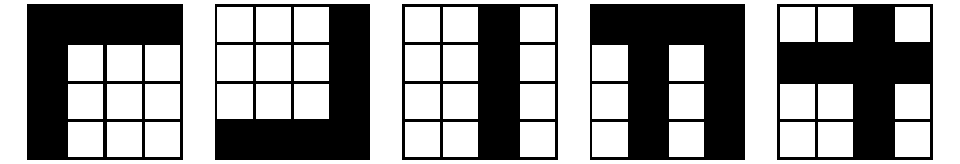
\includegraphics[width=2.8\textwidth, angle=-90]{input_ex.pdf}									
					\end{figure}
				\end{column}
				
				\begin{column}[T]{.9\textwidth}				
				A critical task for a cognitive system is to identify recurring patterns, i.e.\ objects, in a noisy environment, a task that falls under the domain of Independent Component Analysis.
			
				The autonomous activity of the network has no semantic content, being independent from the external world. Meaning can be acquired by correlating sensory signals to specific cliques.
	
				We use the bars problem, in which horizontal and vertical bars are presented on a retina of $L \times L$ pixels. Each of the $2L$ bars is independently drawn with probability $p=1/2L$. Inactive pixels have value $y_l^{\text{ext}}=0$, whereas active pixels always $y_l^{\text{ext}}=1$, even if they are at the intersection of two bars.
											
				Because of this, a \emph{non linear} independent component analysis has to be performed in order to separate bars.
					
				This sensory input layer is connected to every node in the network with excitatory connections $v_{jl}$. At regular intervals the network receives an extra input term:
				\begin{equation*}
					\Delta E_j = \sum_{l=1}^{L^2} v_{jl} y_l^{\text{ext}}
				\end{equation*}
				%The initial weights are chosen so that the average input is $\left\langle \Delta E_j\right\rangle  \approx 0.5$. Larger inputs could inactivate the current winning coalition, and completely drive the network.


			

			\end{column}

			\end{columns}

				

			\end{block}
			
			\begin{block}{Learning rule}
			\begin{columns}
				\begin{column}[T]{.4\textwidth}

					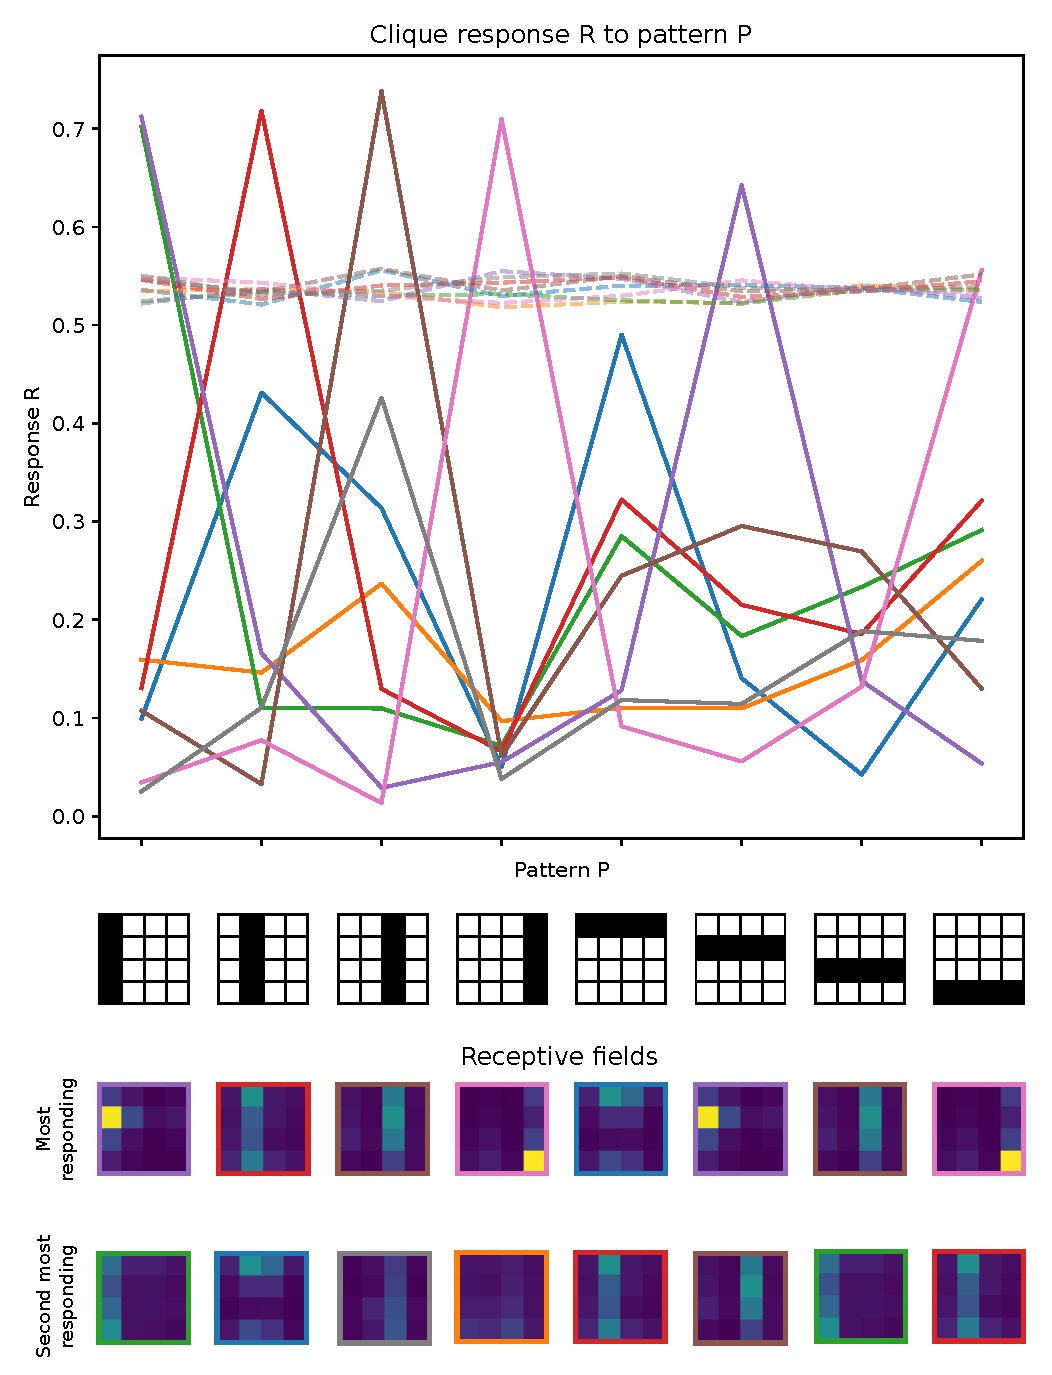
\includegraphics[width=1\linewidth]{complete2.pdf}	
				\end{column}								
				
				\begin{column}[T]{.6\textwidth}
				The learning procedure has to map different bars onto different cliques, by taking advantage of the fact that the sensory input can ``steer'' the competitive dynamics by changing the order of winning cliques.
					
				We employ the following learning rule:
				\begin{gather*}
					\frac{d}{dt} v_{jl} = \left(\dot{y}_j c_j / \tau_v  - 1 / \tau_d\right) y_l^{\text{ext}} v_{jl}  \\
					c_j = \tanh{\left[a \left(V_t - \Delta E_j \right)\right]} \\
					V_t = V^{\text{ina}} + y_j \left(V^{\text{act}} - V^{\text{ina}}\right)\\
					\tau_v \ll \tau_d, \quad V^{\text{ina}} < V^{\text{act}}.	
				\end{gather*}
				We note that:
				\begin{itemize}
					\item the factor $v_{jl}$ ensures that the weights do not change sign,
					\item presynaptic activity $y_l^{\text{ext}}$ is necessary to learning,
					\item $\dot{y}_j$ ensures that learning only takes place when the activity changes significantly,
					\item the term $c_j$ prevents runaway growth or shrinking of weights, with the sliding threshold $V_t$,
					\item the slow decay term $-1/\tau_d$ shrinks non-useful synapses.
				\end{itemize}
				To assess the performance of the learning rule we compute the response $R(\alpha, \beta)$ of clique $\alpha$ to the pattern $\beta$ and the receptive field $F(\alpha, l)$:
				\begin{gather*}
					R(\alpha, \beta) = \frac{1}{S(C_\alpha)} \sum_{\substack{i\in C_\alpha \\ l \in P_\beta}} v_{il} y_l^{\text{ext}} \\
					F(\alpha, l) = \frac{1}{S(C_\alpha)} \sum_{i\in C_\alpha} v_{il}
				\end{gather*}
					
				\end{column}
			\end{columns}
				
			
			\end{block}
			

			\vfill
			\begin{refblock}{References}
			\begin{columns}
 				\begin{thebibliography}{1}
				\begin{column}[T]{.46\textwidth}
					\bibitem{fiser2004modulation}
					Fiser, J., Chiu, C. \& Weliky, M. Small modulation of ongoing cortical dynamics by sensory input during natural vision. Nature 431, 573 (2004).
							
							
					\bibitem{lin2006clique} Lin, L., Osan, R. \& Tsien, J. Z. Organizing principles of real-time memory encoding: neural clique assemblies and universal neural codes. Trends in Neurosciences 29, 48–57 (2006).
																					
				\end{column}
				\begin{column}[T]{.46\textwidth}
					\bibitem{gros2010semantic}
					Gros, C. \& Kaczor, G. Semantic learning in autonomously active recurrent neural networks. Log J IGPL 18, 686–704 (2010).
						
					\bibitem{tsodyks2008model}
					Mongillo, G., Barak, O. \& Tsodyks, M. Synaptic Theory of Working Memory. Science 319, 1543–1546 (2008).
						
				\end{column}
 				\end{thebibliography}
			\end{columns}
			\end{refblock}
		%\vfil
		%%% END CONTENT of column 2 %%%


		} % end of parbox
		% ---------------------------------------------------------%
		% end the column
		\end{minipage}
		%\end{beamercolorbox}
	\end{column}
	% ---------------------------------------------------------%
	% end of column 2
\end{columns}
\hfill
\vskip1ex
\end{frame}
\end{document}
